\documentclass[tikz,border=2mm]{standalone}

\usepackage{pgfplots}
\pgfplotsset{compat=1.18}
\usepackage{xcolor}

% ---------- Axis style ----------
\pgfplotsset{
  myaxis/.style={
    width=8.2cm,
    height=6.2cm,
    xmin=0, xmax=1,
    xlabel={Observed missingness proportion},
    ylabel={MSE},
    axis lines=left,
    axis line shift={4pt},
    tick label style={font=\small},
    label style={font=\small},
    title style={font=\small},
    legend style={
      font=\small,
      draw=none,
      fill=none
    }
  }
}

% ---------- Colors ----------
\definecolor{ps}{RGB}{27,158,119}
\definecolor{ccs}{RGB}{217,95,2}
\definecolor{mle}{RGB}{117,112,179}
\definecolor{mlemi}{RGB}{231,41,138}
\definecolor{mi}{RGB}{102,166,30}
\definecolor{mimi}{RGB}{230,171,2}
\definecolor{refMU}{RGB}{166,118,29}
\definecolor{refMC}{RGB}{102,102,102}

% ---------- Plot styles ----------
\pgfplotsset{
  datapoints/.style={
    only marks,
    mark=*,
    mark size=0.55pt,
    opacity=0.22
  },
  loessline/.style={
    very thick
  }
}

% ---------- Fake point cloud ----------
\newcommand{\fakepoints}[2]{%
  \addplot[
    datapoints,
    draw=#1,
    fill=#1
  ]
  coordinates {
    (0.00,#2) (0.05,#2) (0.10,#2) (0.15,#2) (0.20,#2)
    (0.25,#2) (0.30,#2) (0.35,#2) (0.40,#2) (0.45,#2)
    (0.50,#2) (0.55,#2) (0.60,#2) (0.65,#2) (0.70,#2)
    (0.75,#2) (0.80,#2) (0.85,#2) (0.90,#2) (0.95,#2)
    (1.00,#2)
  };
}

% ---------- Fake smooth curve ----------
\newcommand{\fakeline}[2]{%
  \addplot[
    loessline,
    color=#1
  ]
  coordinates {
    (0.0,#2)
    (0.2,{#2 + 0.01})
    (0.4,{#2 + 0.02})
    (0.6,{#2 + 0.04})
    (0.8,{#2 + 0.07})
    (1.0,{#2 + 0.10})
  };
}

\begin{document}

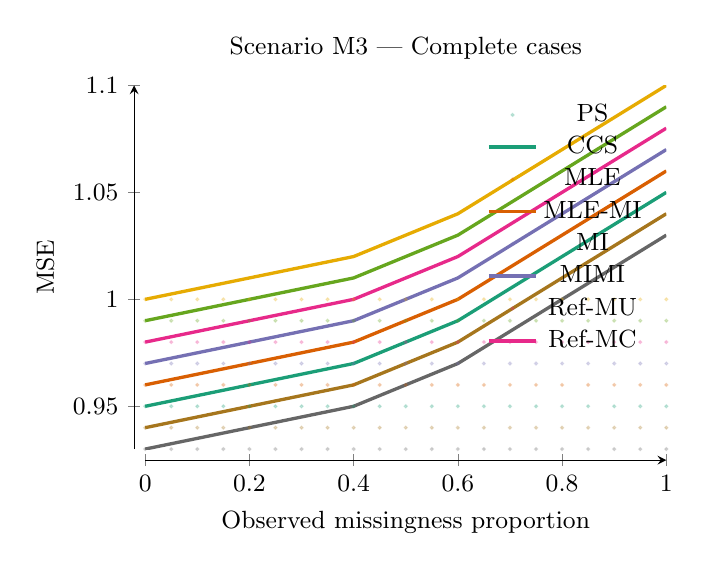
\begin{tikzpicture}
\begin{axis}[myaxis, title={Scenario M3 — Complete cases}]

  \fakepoints{ps}{0.95}
  \fakeline{ps}{0.95}
  \addlegendentry{PS}

  \fakepoints{ccs}{0.96}
  \fakeline{ccs}{0.96}
  \addlegendentry{CCS}

  \fakepoints{mle}{0.97}
  \fakeline{mle}{0.97}
  \addlegendentry{MLE}

  \fakepoints{mlemi}{0.98}
  \fakeline{mlemi}{0.98}
  \addlegendentry{MLE-MI}

  \fakepoints{mi}{0.99}
  \fakeline{mi}{0.99}
  \addlegendentry{MI}

  \fakepoints{mimi}{1.00}
  \fakeline{mimi}{1.00}
  \addlegendentry{MIMI}

  \fakepoints{refMU}{0.94}
  \fakeline{refMU}{0.94}
  \addlegendentry{Ref-MU}

  \fakepoints{refMC}{0.93}
  \fakeline{refMC}{0.93}
  \addlegendentry{Ref-MC}

\end{axis}
\end{tikzpicture}

\end{document}
